%%%%%%%%%%%%%%%%%%%%%%%%%%%%%%%%%%%%%%%%%%%%%%%%%%%%%%%%%%%%%%%%%
\chapter{SMART SPREADING FACTOR TECHNIQUE}\label{ch:proposed_technique}
%%%%%%%%%%%%%%%%%%%%%%%%%%%%%%%%%%%%%%%%%%%%%%%%%%%%%%%%%%%%%%%%%

The collision problem illustrated in Figure \ref{fig:collision} is solved by forcing some of the close nodes to select higher spreading factors even though they are able to communicate with lower spreading factors. This has the potential to prevent collisions due to the orthogonality of the spreading factors as shown in Figure \ref{fig:collision_solution_single_gw}. Higher spreading factor assigned nodes are drawn with bold circle border in Figure \ref{fig:collision_solution_single_gw}. However, the distribution of spreading factor among nodes becomes an important problem. Increasing a node's spreading factor should be done carefully since higher spreading factor means longer air time and longer air time means increasing the probability of collisions with other high spreading factor transmissions. In multiple gateways scenarios, this approach may increase the collisions with the nodes in other gateways' range. Thus, extra care should be taken for nodes in the intersection area of the gateways illustrated in Figure \ref{fig:collision_solution_multi_gw}.

\begin{figure}
\centering
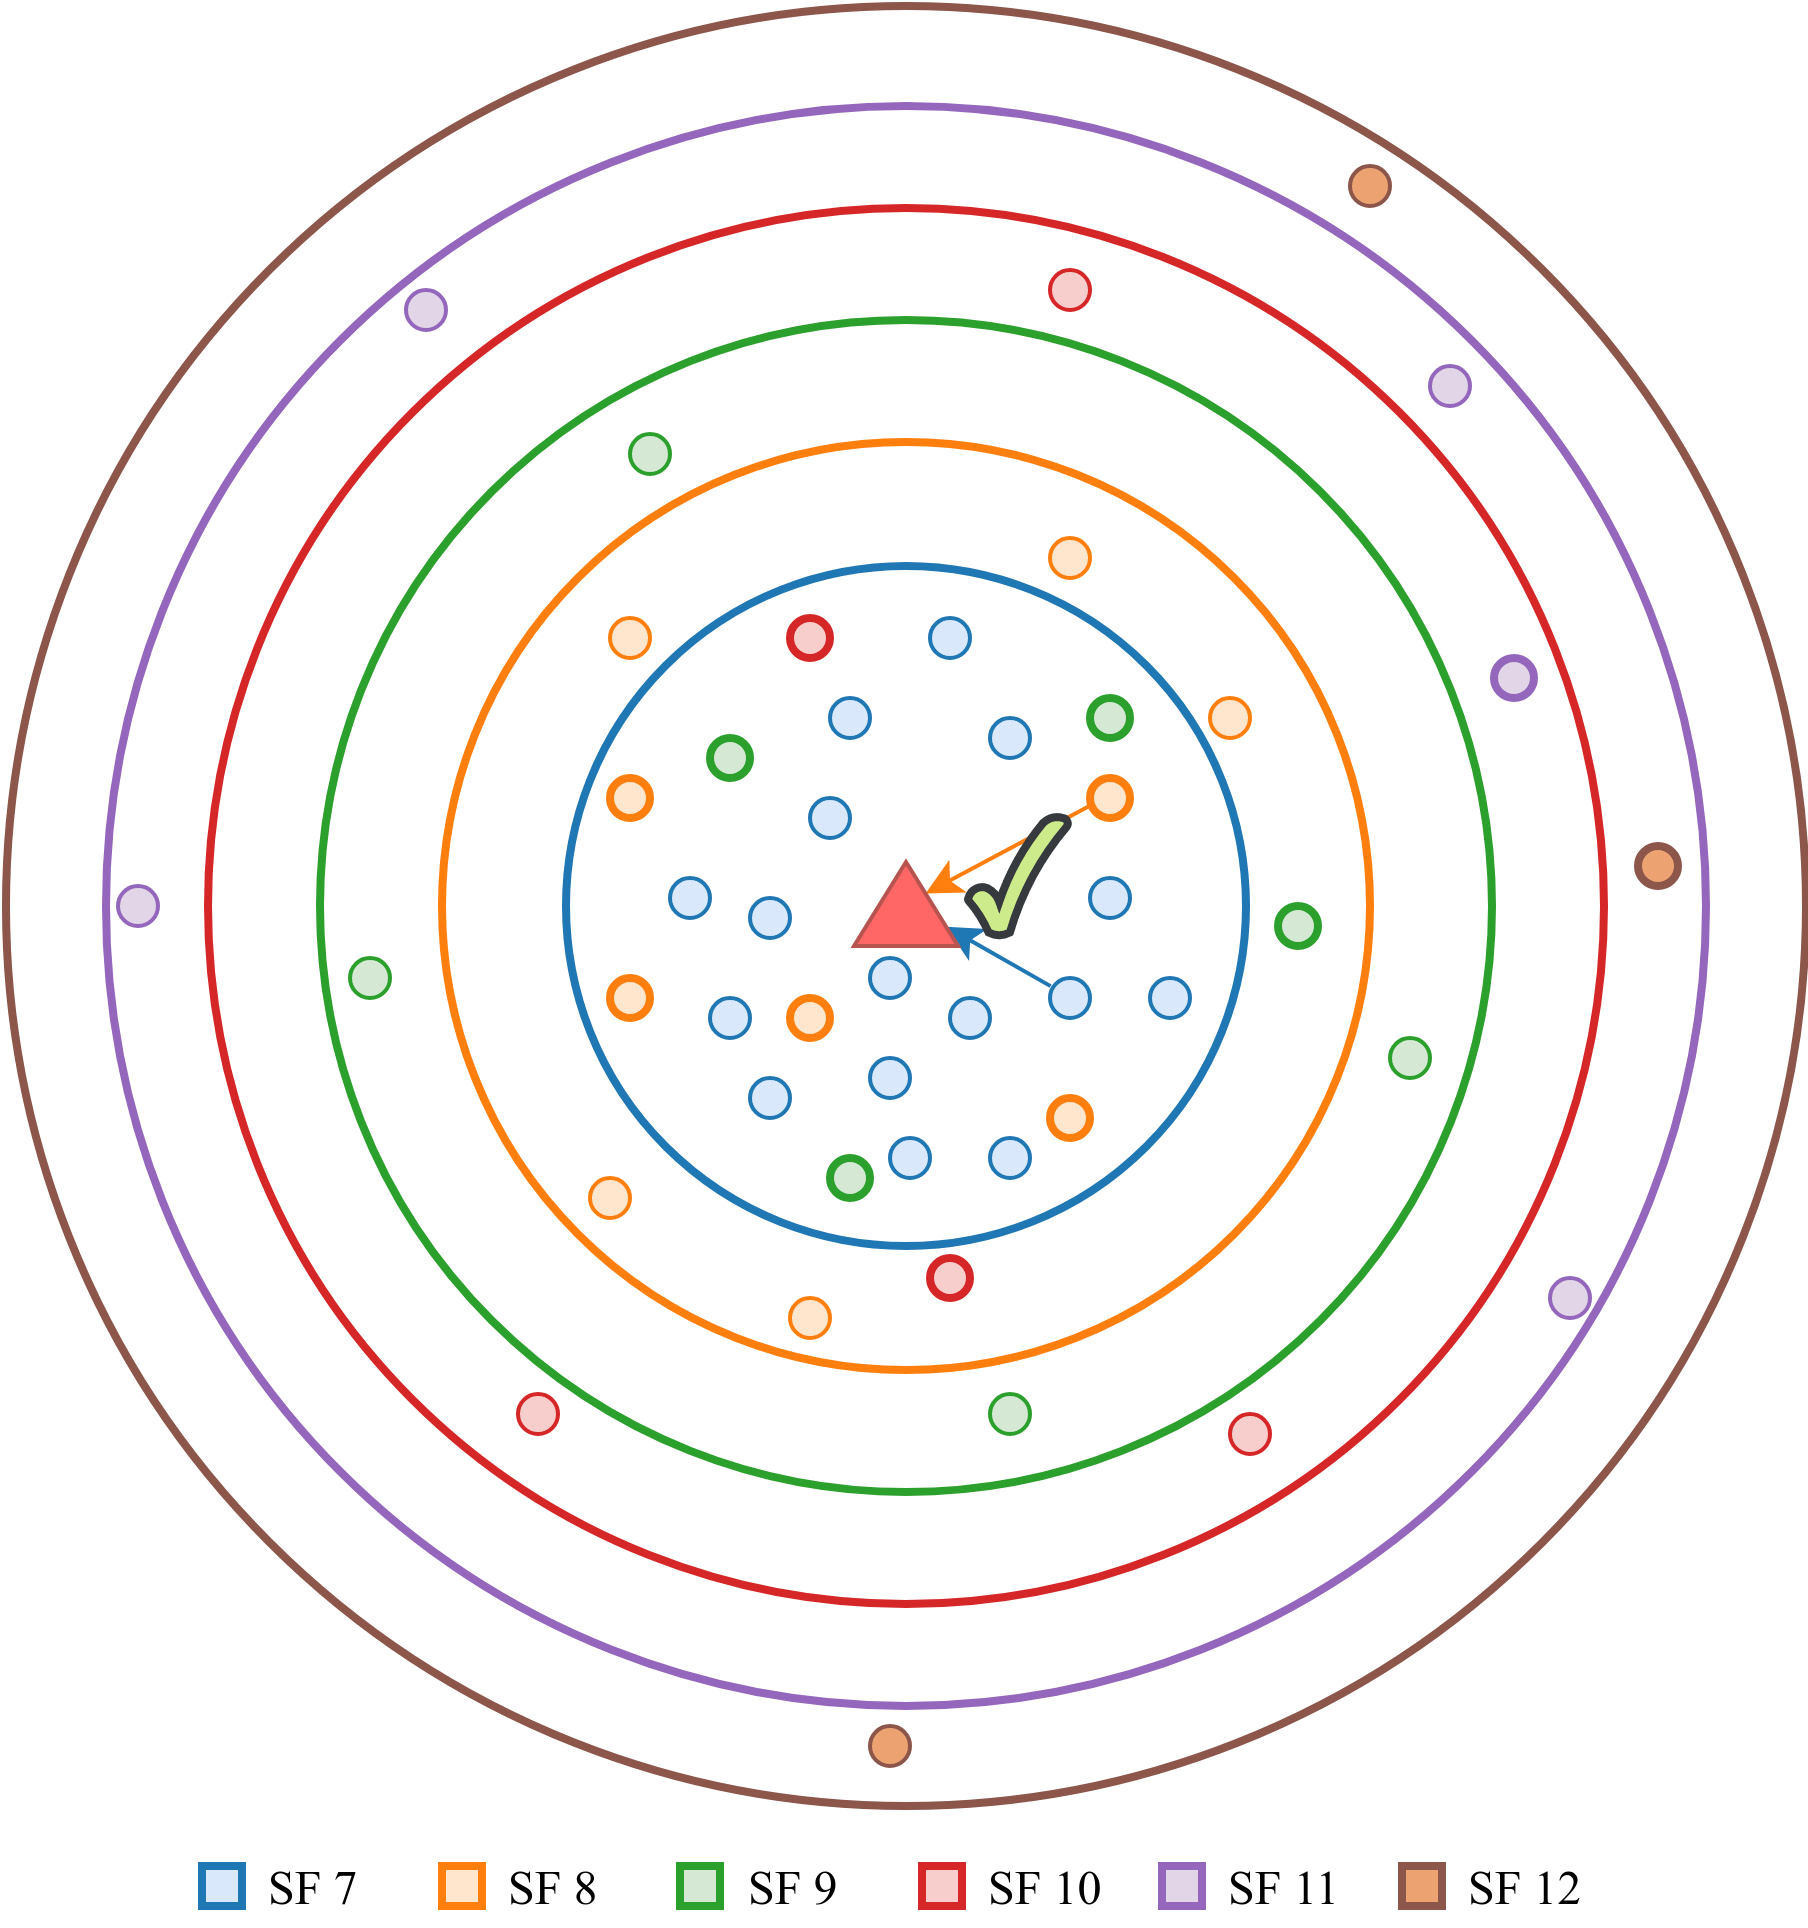
\includegraphics[width=.7\linewidth]{fig/lora_single_gw_collision_fix.png}
\vspace*{5mm}
\caption{Collision avoidance by using higher spreading factor for nodes close to the gateway.}
\label{fig:collision_solution_single_gw}
\end{figure}

\begin{figure}
\centering
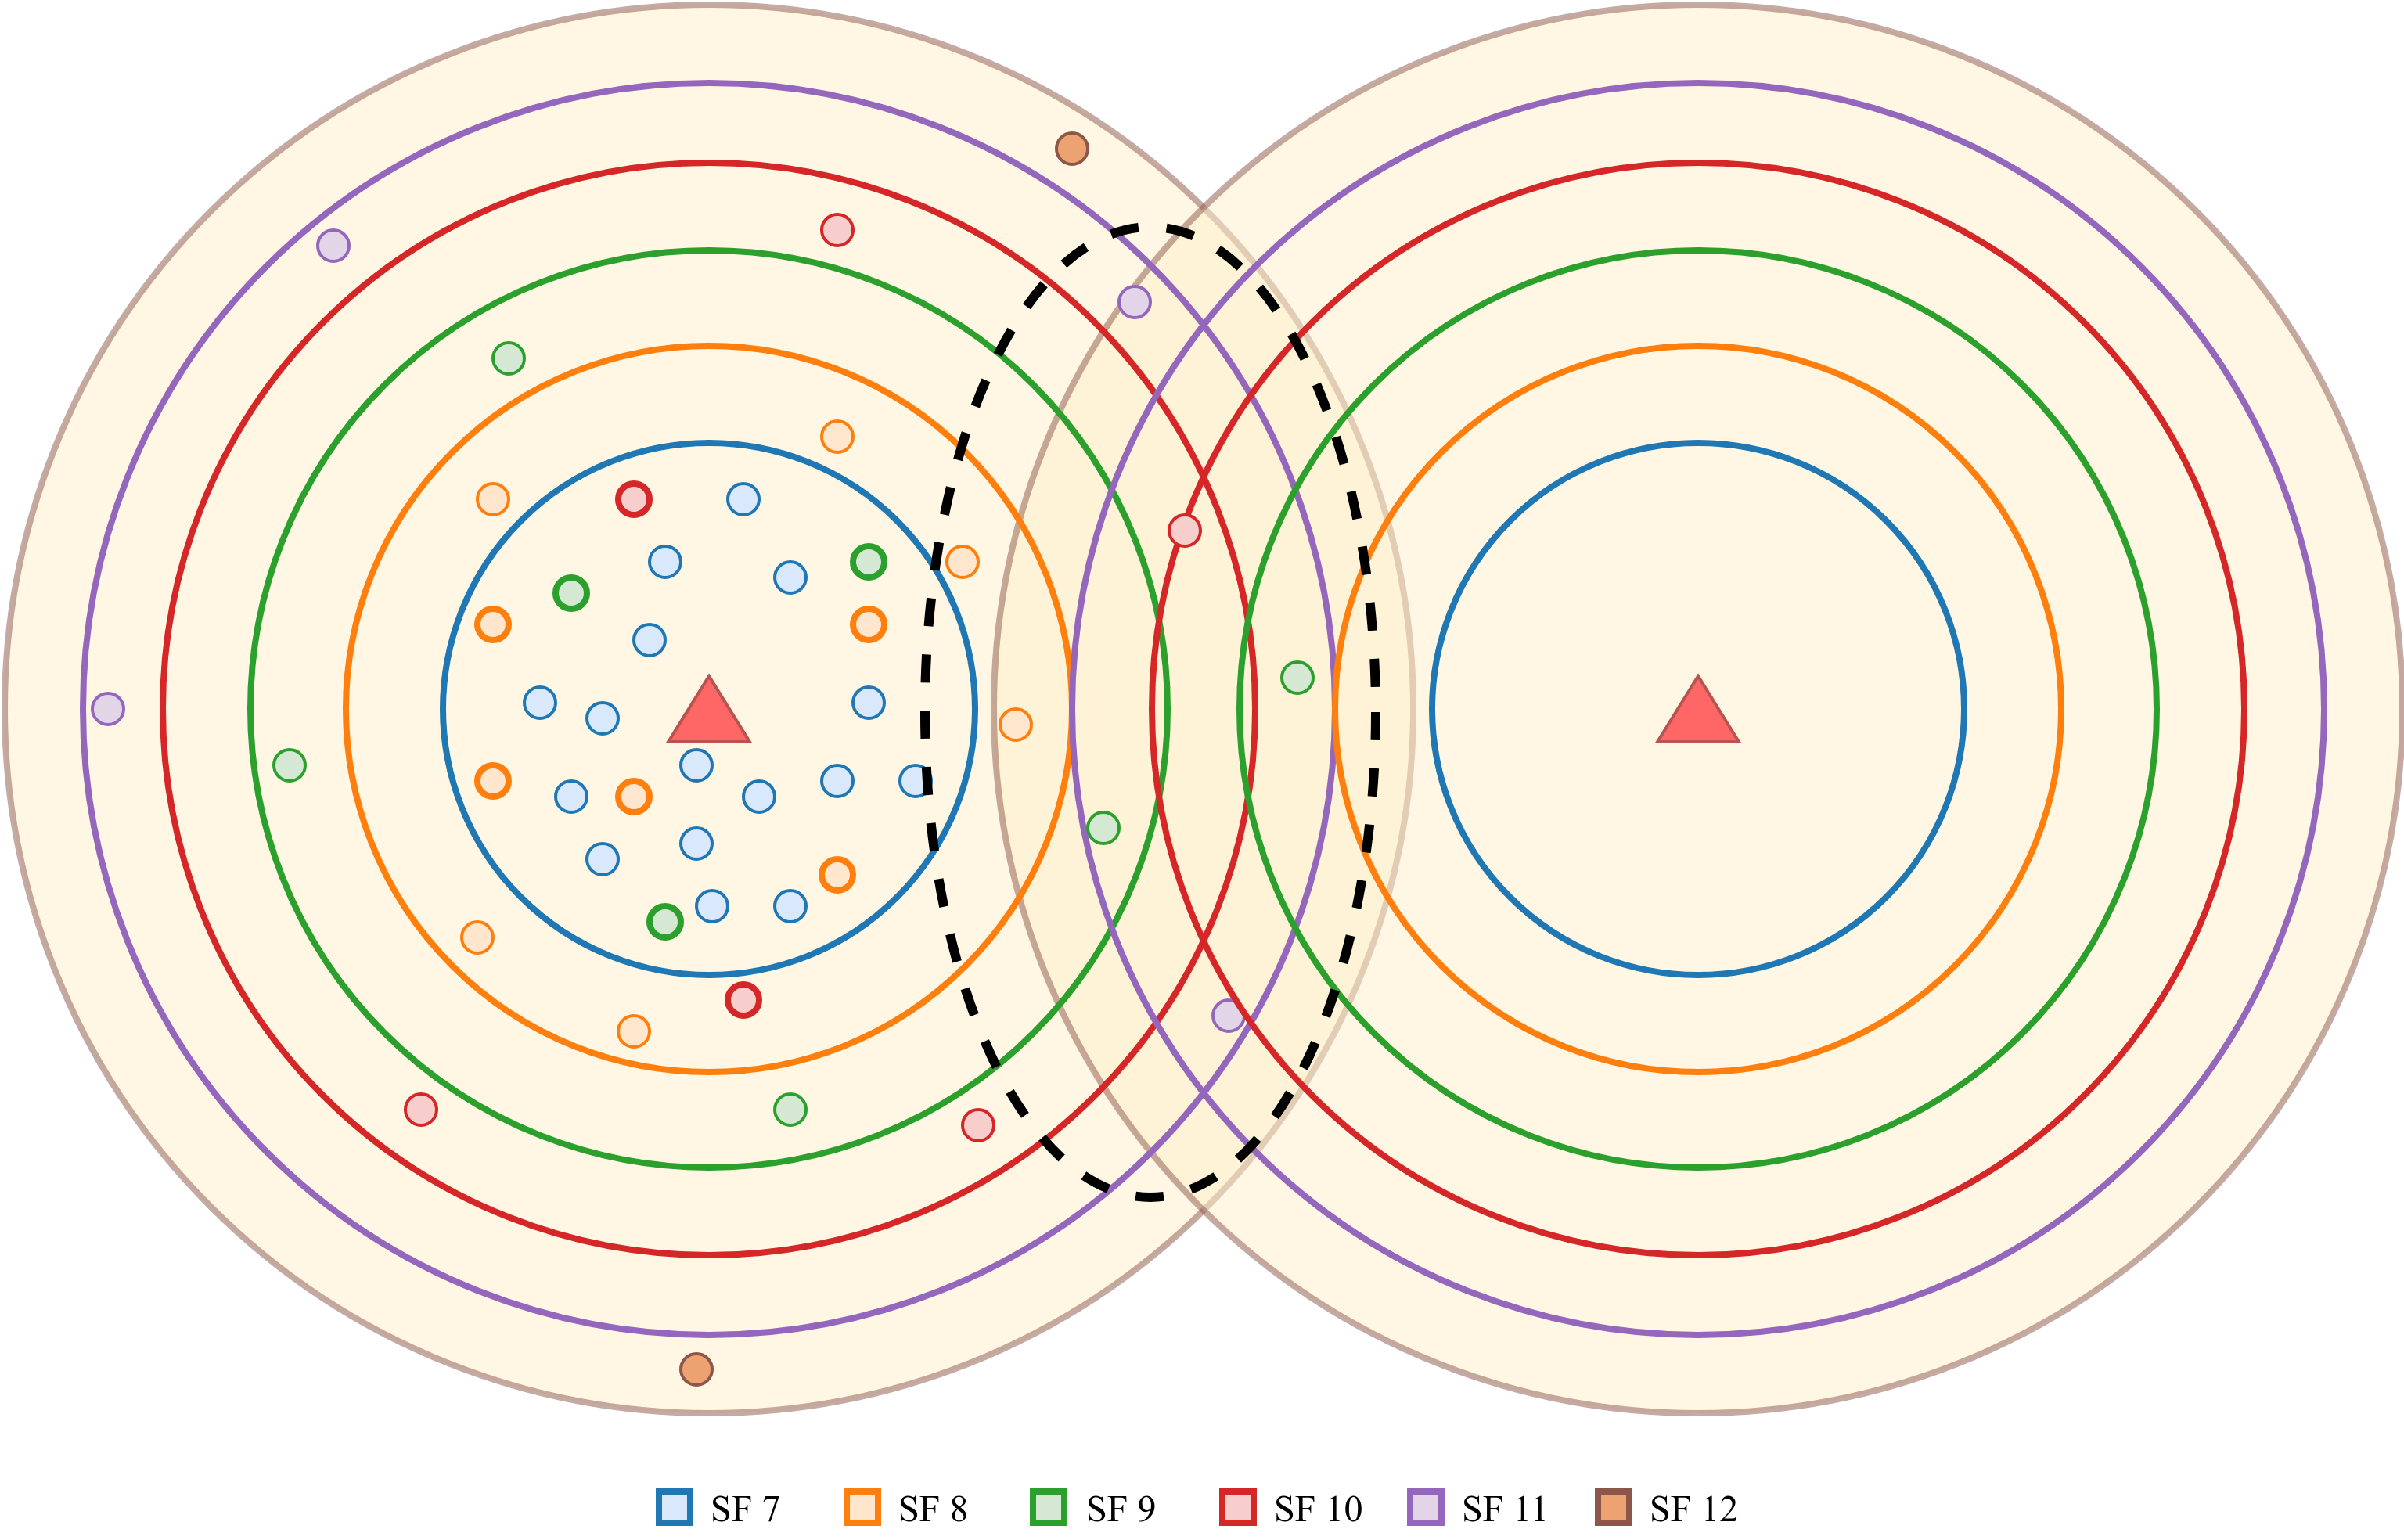
\includegraphics[width=\linewidth]{fig/lora_multi_gw_collision_fix.png}
\vspace*{4mm}
\caption{Collision avoidance for intersecting gateways.}
\label{fig:collision_solution_multi_gw}
\end{figure}

It is difficult to propose a single spreading factor assignment rule for every possible LoRaWAN topology since every network is different and optimizing their nodes' spreading factors requires different rules. For this reason, machine learning based spreading factor assignment approach is proposed to decrease the collisions for the same spreading factor transmissions. This technique starts by learning the transmission behavior of the nodes in a network. NS can keep track of successful uplink transmissions and their spreading factors. NS can also keep track of some of the collided transmissions if header part of the packet is not interfered at the gateway. However, NS cannot keep track of transmissions with lower receive power than the sensitivity of the gateway. Using those obtained information, NS can train a classifier to predict future transmission result for a specific node and a specific spreading factor. Using this prediction model NS can assign spreading factors to nodes considering the collision probability. NS can modify spreading factor of the node using existing ADR mechanism. Thus, this technique does not require any modification on LoRaWAN protocol. It is reasonable to assume that every end node makes at least one uplink transmission in a day, so there is at least one open receive window every day to inform end nodes about new spreading factor.

In this work, DTC and SVM \cite{Alpaydin} schemes are employed to predict the transmission results. Class weights are balanced according to sample distributions for both methods. For DTC, Gini impurity criteria is used to measure the quality of splits. For SVM, penalty parameter is set to 1, degree is set to 3 and RBF kernel is used.

It is possible to generate mass amount of LoRaWAN transmission logs for various topologies using our simulator. Training dataset size is directly proportional to simulation duration. Thus, increasing the simulation duration, improves the prediction accuracy up to some extent. In real world deployments, NS can keep track of transmissions and it can create a classifier daily basis. Then, gateways can request from nodes to use suggested spreading factors.

There are three features in the dataset generated by the simulation tool. Features of the dataset are: X coordinate of the transmission source, Y coordinate of the transmission source and spreading factor of the transmission. X and Y coordinate feature values are continuous numbers. In this technique, it is assumed that node locations are known to NS by triangulation. Spreading factor feature values are integer numbers between 7 to 12. Class label of the dataset is the result of the transmission. Class label values are successful, interfered and under sensitivity. Example dataset can be found in Table \ref{table:dataset}. DTC and SVM prediction schemes are integrated into the simulation tool to study smart spreading factor assignment schemes. A classifier is trained from generated dataset and this classifier is used for selecting optimum spreading factor for the nodes in the network.

\begin{table}
\centering
\caption{Sample section of a transmission dataset.}
\label{table:dataset}
\begin{tabular}{|c|c|c|c|}
\hline
\textbf{X Coordinate} & \textbf{Y Coordinate} & \textbf{Spreading Factor} & \textbf{Result} \\ \hline
      -2033.1  &  713.0  &   8   &   successful \\ \hline
       995.5   & -2148.6 &   7   &   under sensitivity \\ \hline
      -3738.6  & -4665.3 &   12  &   interfered \\ \hline
      -1268.9  &  1348.2 &   9   &   successful \\ \hline
      -427.1   &  593.7  &   9   &   successful \\ \hline
      -193.4   & -4047.5 &   11  &   interfered \\ \hline
      -2729.1  & -3663.3 &   10  &   interfered \\ \hline
       637.3   & -715.3 &   7   &   successful \\ \hline
       3843.7  &  1996.3 &   8   &   successful \\ \hline
       2853.6  & -2696.0 &   7   &   successful \\ \hline
      ...      & ...     &   ... &   ... \\ \hline
\end{tabular}
\end{table}

The tool first runs a simulation with random spreading factor scheme. After random spreading factor scheme simulation completed, transmission logs are combined into three feature columns and one class label column to create the training dataset. Then, the dataset is fed to Python scikit-learn DTC or SVM classifiers for training phase. After the classifier model is built, second simulation is run with the trained classifier. The tool selects optimum spreading factor for transmissions considering prediction of the transmissions. For every transmission, the classifier predicts the transmission result for the lowest possible spreading factor. If the transmission result is predicted as interfered, then the tool increases the spreading factor and predicts a new transmission result. If the new transmission result is classified as successful, then simulator continues to execute with selected spreading factor. If no spreading factor transmission result is predicted as successful, then the tool selects the lowest possible spreading factor and continue to execute.
